\documentclass[a4paper, 12pt]{article}
\usepackage[top=2.5cm, bottom=2.5cm, left=2.5cm, right=2.5cm]{geometry}
\usepackage[utf8]{inputenc}
\usepackage[T1]{fontenc}
\usepackage{indentfirst}
\usepackage{tabularx}
\usepackage{graphicx}
\usepackage{color}
\usepackage{amsmath}
\usepackage{amssymb}
\usepackage{titling}
\usepackage{float}
\usepackage{geometry}
\usepackage[final]{pdfpages}
\newcommand{\ii}{\textit}
\setcounter{tocdepth}{2}


%\title{Impact of network topology on opinion dynamics in a bounded confidence model}
%\author{Artur Przybyłek}

\begin{document}

\includepdf{/home/arti/studia/python/praca_magisterska/tex/praca_dyplomowa_strona_tytulowa_en.pdf}
\newpage
\includepdf{/home/arti/studia/python/praca_magisterska/tex/praca_dyplomowa_strona_tytulowa_pl.pdf}
\newpage

%\begin{titlepage}
%	\maketitle
%	\begin{abstract}
%	In this work we will investigate the impact of a social network topology on a process of opinion spreading in a bounded confidence model. We will conduct Monte Carlo simulations on various model networks and study distributions of final opinions, dynamics of changes, fragmentation of opinions, time of relaxation and establishing of consensus. We will show that the course of the dynamics process, as well as its final state vary depending on network's structure, size and connection density.
%	\end{abstract}
%\end{titlepage}


\tableofcontents

\newpage

\section{Introduction}


People opinions on a given issue may vary a lot depending on their own beliefs, the environment of living or acquired knowledge. Sometimes a person change his opinion due to some facts that he was not aware of earlier, his own new impressions on a given subject or the social pressure exerted by his surrounding. Psychological aspects play very important role in the process of opinion dynamics in community. From observation of humans we can spot some types of behavior, such as conformity, acting independently or disagreement, which are then used in constructing models for simulating process of opinions dynamics in social networks. Often the agent--based modeling is used for that purpose \cite{sp}.

There are numerous models that can be applied to various cases of opinion evolution, in which human interactions play very important role. For example, one could think of voting in referendum, when opinion can be described by two states ("yes" or "no"). To this case the $q$--voter model may be applied \cite{qv}. Basic idea behind the model is that voters can change their opinions influenced by group of others (i.e. conformity). 
\indent

Another examples of models developed for the purpose of opinions dynamics, in which agents can choose between two opposite opinions, are majority rule (MR) model \cite{mr} and Sznajd model \cite{sm}. In MR model agents accept opinion shared by majority of their influence group. This property causes that the model is suitable for being applied to public debates. In Sznajd model agents act as conformists or non--conformists depending on unanimity of a given pair of neighbors.
\indent

All of the models mentioned above could be useful to study the process of opinions evolution in some community. Basic assumption for these models is that an agent can decide between exactly two opinions. However, sometimes an opinion can not be considered in categories of "black or white", but instead many shades of gray are possible. We can say for instance "I think that their chances to win the tournament are 30\%." or "In my opinion we should look for cheaper option on vacations.". These sentences represent opinions which do not fall into "0 or 1" pattern. A political opinion of an individual is another good example because it might be "more to the left" or "more to the right". In order to model opinion dynamics of such opinions we should use a continuous opinion space.
\indent

Such continuous space was used for instance in the Deffuant model \cite{dm}. The main idea in this model is that if opinions of two agents are similar, then they adjust their opinions to each other. The model parameter which regulates how eager are agents to rely on others is called confidence level. Similar agents behavior can be observed in bounded confidence (BC) model proposed by Hegselmann and Krause \cite{bc}. In BC model agents adjust their opinions not only to one neighbor but to all neighbors whose opinions are similar (in terms of confidence level), hence the model may be applied to public debates and talks on forum when participants of the meeting express their opinions and try to find common solution on a given problem.
\indent

In this work we want to investigate opinion dynamics in BC model. We should remember that dynamics of agents' opinions depends not only on the model properties but also on structure of the network. In real life situations, for example on public debates or fore, we often know about opinions of few other people and not necessary the whole group. This fact could have crucial meaning in terms of our attitude. In order to find out what influence does connectivity between agents has on their behavior, we will consider various network topologies which could be applied as an underlying structure for the model. We will study not only the dynamics of agents opinions changing in network, but also typical final states of opinions evolution process for given confidence levels, especially investigating cases when consensus is being established.

\section{Network topologies}
In order to simulate opinion dynamics process in a given community, we have to carefully choose network topology first. We will investigate various topologies, thus different networks, in which the process of changing opinions takes place, may differ in terms of their structure. For instance, in one community, we could have centralized network topology, while in another one, network may have regular ring topology. The dynamics of changing opinions, as well as final state of agents' opinions, may be different in these 2 networks, because of different structure of connections between agents. Throughout this work we choose to investigate 3 types of network topologies, which nicely reflect some properties of real--life communities:
\begin{itemize}
\item complete graph (CG) \cite{cg},
\item Watts--Strogatz graph (WS) \cite{ws},
\item Barabasi--Albert graph (BA) \cite{ba}.
\end{itemize}
All of these topologies could be applied to simulate the structure of different types of communities. We plot examples of these model networks in Fig. \ref{nets}.

\begin{figure}[H]
		\centering
		\includegraphics[width=\textwidth]{/home/arti/studia/python/praca_magisterska/plots/all_nets.pdf}
		\caption{Example networks of various topologies.}
		\label{nets}
\end{figure}

In Fig. \ref{nets} we could see networks' parameters, such as: $n$, $k$, $p$, $m$. Their meaning is as follows:
\begin{itemize}
\item $n$ -- the number of agents in a network,
\item $k$ -- the number of initial connections for every agent in a network,
\item $p$ -- the probability of changing an agent' neighbor to randomly chosen, not yet connected agent,
\item $m$ -- the number of new connections created in a network, when new agent is being attached.
\end{itemize}

\subsection{Complete graph}
In a complete graph any chosen agent is connected with all other agents (see left--most graph in Fig. \ref{nets}). Thus, when complete graph is network topology for BC model, a lot of agents can influence opinion of a chosen agent at once. In advance, very nice property of complete graph network is that an agent take into account the opinions of the whole community, which gives him a wide spectrum of others' opinions and may be helpful in adjusting his own opinion to them. 
\indent

Because of the assumption of fully--connected network, this topology may be applied for some small discussion groups where everybody shares own point of view. Another use case, for bigger group sizes, might be opinion forming by non--verbal transmission. For example, we could change our opinion on what is now trendy in fashion by looking on what clothes do others wear.

\subsection{Watts--Strogatz network}
In Watts--Strogatz model every agent has initially the same number of connections $k$ and is connected with $\frac{k}{2}$ closest agents on the left and $\frac{k}{2}$ closest agents on the right. Then, every agent can change every of his neighbor to other agent in different graph region with probability $p$ (see central graph in Fig. \ref{nets}). As the result of changing neighbors, only the structure of connections in a network changes, while the number of all connections in a network remains the same. However, after changing initial neighbors, some agents may have a little more connections and some a little less.
\indent

Typically, the model network is constructed with $n\gg k \gg \log[n] \gg 1$ and $0 \leq p \leq 1$. When $p=0$ network has regular ring topology with none of the agents changing his neighbor, whereas $p=1$ leads to fully--random connections in network.

When agents change their neighbors not too often ($0.1 \leq p \leq 0.5$), then the model has the so--called small--world property. Small--world property means that agents tend to be mostly connected with their closest surrounding, but at the same time the  closest path between two randomly chosen agents in network is small. This property nicely reflects connections in some communities. As an example we could think of children participating to the same school. Children know each other well within their class, but have also some contacts outside it. Thus, the friendship chain connecting two children from different classes should not be long.

\indent
Another property of Watts--Strogatz graphs is that they have non--centralized structure (especially when $p$ is small). Average number of agents' connections is equal to $k$ and typically there are no such agents in network, who would have been connected with much more agents than others. Thus, opinions transmission between two randomly chosen agents might take some time.

\indent
We could think of opinions spread in our living neighborhood or at round--table meeting as Watts--Strogatz model use cases to BC model.

\subsection{Barabasi--Albert network}
Barabasi--Albert network is constructed from initially fully--connected network of $m_0$ agents and then by iteratively attaching new agents with $m$ new connections (for the simulations purposes we will take $m_0=m$). New connections are created from new agent to one of agents already being in the network. New agent's preference for which agent to choose is proportional to number of connections that given agent already has. This manner typically leads to formation of a few hubs -- agents who have a lot of connections, we might call them central agents in the network (see right--most graph on Figure \ref{nets}). This property implies more central structure in the network. These hubs may influence many other agents in terms of changing opinions. We may think of them as celebrities, which are well--known in community. 

\indent
We could think of Internet communities such as social medias and forums as a good example of networks with similar topology. Also political parties or some companies in which a few individuals who are highest in the hierarchy are the most influential ones, may be considered as networks similar to Barabasi--Albert model.

\section{Bounded Confidence model}

The basic idea behind Bounded Confidence (BC) model \cite{bc} is that agents interact with others who have similar opinions and customize their own opinions slightly to them. Interaction is not possible if two opinions differ too much. The model parameter, i.e. confidence level $\epsilon$ gives us information how much agents rely on others. If confidence level is small, then agents act like non--conformists, sticking to their own opinions. On the other hand, when confidence level is big, agents are more open for discussion and take into account others points of view, acting more like conformists.
\indent

The confidence level might take different values, when applied to opinion dynamics processes. For example, when political party wants to state their position on a given issue, confidence level should be big in order to achieve consensus -- one common opinion. For the case of smaller confidence level we could think of political discussion on family meeting, people then express their opinions, but it is rather rare that they would change their mind strongly by being influenced by others.
\indent

In BC model we assume that agents opinions can be described as a number in the interval $[0, 1]$. Opinion $0$ is the left--most and $1$ is the right--most. Many variants of intervals of confidence levels could be considered (for instance asymmetric confidence levels or various confidence levels assigned individually to agents). In this work we will investigate only the case of symmetric ones, following the KISS principle ("Keep it simple, stupid") \cite{kiss}. Symmetric confidence levels means that $\epsilon$ is the same for all agents and also equal on the left side and on the right side ($\epsilon_l=\epsilon_r=\epsilon$). 
\indent

We introduce the BC model with symmetric confidence levels, using asynchronous random updating schema \cite{sai}, as it nicely reflects appearance of social interactions. 
\indent

The time is measured by Monte Carlo steps (MCS). Which of them is composed of $n$ elementary time steps $dt=\frac{1}{n}$. 

\indent
We will denote by $x_i(t)$ the opinion of agent $i$ in time $t$. Then, algorithm for the BC model is as follows:

\begin{enumerate}
\item Set time: $t \rightarrow 0$.
\item Repeat $n$ times the following procedure:
	\begin{enumerate}
	\item Choose randomly agent $i$.
	\item Set opinion of agent $i$ in time $t+dt$ according to the equation:
	\begin{equation}
	x_i(t+dt) = \left| I(i, x_i(t)) \right|^{-1} \sum_{j \in I(i, x_i(t))} {x_j(t)},
	\label{bceq}
	\end{equation}
	where $I(i, x_i(t)) = \{1 \leq j \leq n: \left| x_i(t) - x_j(t) \right| \leq \epsilon \}$.
	\item Increase time: $t \rightarrow t + dt$
	\end{enumerate}
\item If for any agent $1 \leq i \leq n$: $|x_i(t) - x_i(t-1)| > 0.001$, then go back to step 2.
\end{enumerate}
\indent

When an agent changes his opinion, he accepts average opinions of all his neighbors who have similar opinions in terms of confidence level together with himself. It may happen that in one MCS of simulation (composed of $n \cdot dt$ small steps), one agent will be influenced to change his opinion few times, while other agent will not be influenced at all. Simulation of the model is finished when none of the agents changes his opinion by more than 0.001 in one MCS.


\section{Simulations}

\subsection{Simulations methodology}
Our goal of simulations is to compare how different values of network size $n$, parameters $k$, $p$, $m$ and also confidence level $\epsilon$ affect the process of opinions dynamics, especially its final state. We also want to extract main differences in results between investigated network topologies. In our study we will investigate various ranges of parameters:

\begin{itemize}
\item $n$ ranging from $100$ to $500$ (also $n=50$ for the purpose of showing single trajectories),
\item $k$ ranging from $4$ to $12$ and also from $10$ to $50$,
\item $p$ ranging from $0.1$ to $0.5$,
\item $m$ ranging from $2$ to $10$,
\item $\epsilon$ ranging from $0.01$ to $0.4$.
\end{itemize}

Before each simulation of the model we will take new instance of underlying network and set of random agent opinions from uniform distribution $\mathcal{U}(0, 1)$. Then, we will perform Monte Carlo simulation of the model with symmetric confidence levels and asynchronous random updating.
\indent

 In order to obtain reliable results, for each set of network parameters and confidence level, we will perform 100 Monte Carlo simulations of the model and then calculate average results.
\indent

Having the results of performed simulations, we will be able to study such features as:
\begin{itemize}
\item distribution of final opinions
\item impact of confidence level for reaching consensus
\item dynamics of opinions changes
\item fragmentation of opinions
\item relaxation time
\end{itemize}
\indent

We will conduct simulations on the machine with dual--core 1.8 GHz processor: AMD E2-3000M APU. We will use Python 3.6.4 programming language.

\subsection{Time evolution of opinions}

In order to see how opinions change through time, we will plot agents opinions against time for several single simulation runs of BC model. We will do this for 4 different values of the confidence level: $\epsilon=0.05, 0.15, 0.25, 0.35$ using different underlying network topologies.

\subsubsection{Complete graph}

\begin{figure}[H]
		\centering
		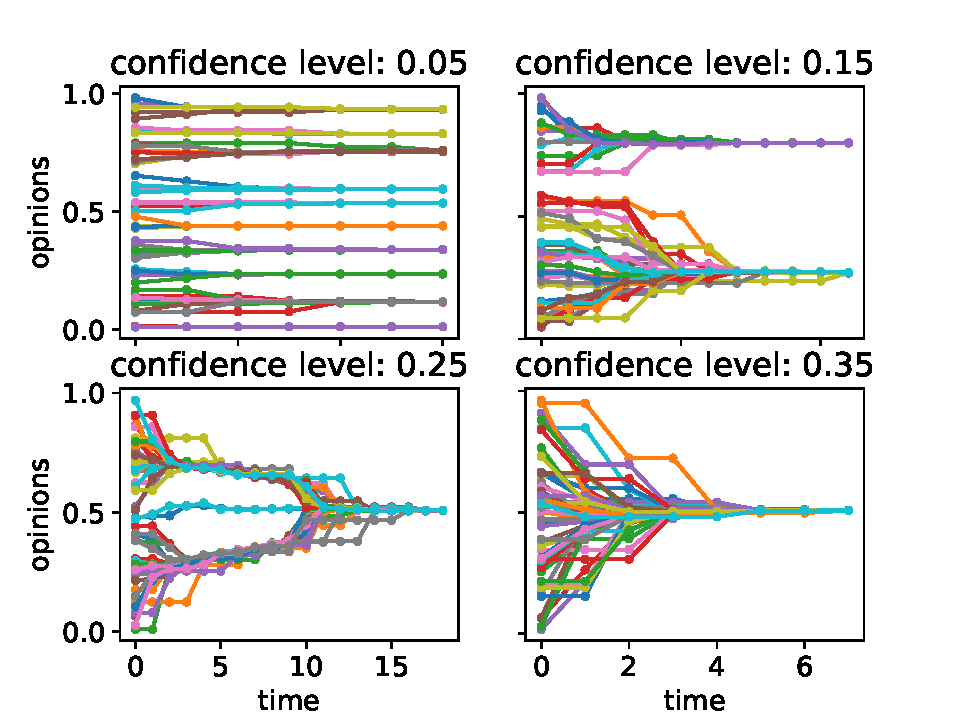
\includegraphics[width=\textwidth]{/home/arti/studia/python/praca_magisterska/plots/single_cg_50.pdf}
		\caption{Opinions dynamics for complete graph network with $n=50$ and various confidence levels.}
		\label{f2}
\end{figure}
As we can see in Fig. \ref{f2}, for higher values of confidence level ($\epsilon=0.25, 0.35$) at the end of simulation asymptotic state of opinion dynamics was the same. In both cases agents reach consensus, but the way of establishing was different.
We can see that for confidence level $\epsilon=0.25$ in first phase two big clusters were formed with one small between them, opinions were mainly polarized. Then, in second phase of dynamics, clusters merged in one. Network experienced phase transition, a rapid transformation from one state to another, in this case from polarization to consensus. On the other hand, for $\epsilon=0.35$ agents from the beginning of simulation aimed to share one common opinion.
\indent


For small confidence level ($\epsilon=0.05$) there occurs fragmentation of opinions -- 11 clusters are formed and for confidence level $\epsilon=0.15$ opinions dynamics leads to a fragmentation into 3 clusters.
\indent

In most cases, biggest changes of opinions occur in early phase of the simulation, excluding discussed phase transition for $\epsilon=0.25$.

\subsubsection{Watts--Strogatz}

\begin{figure}[H]
		\centering
		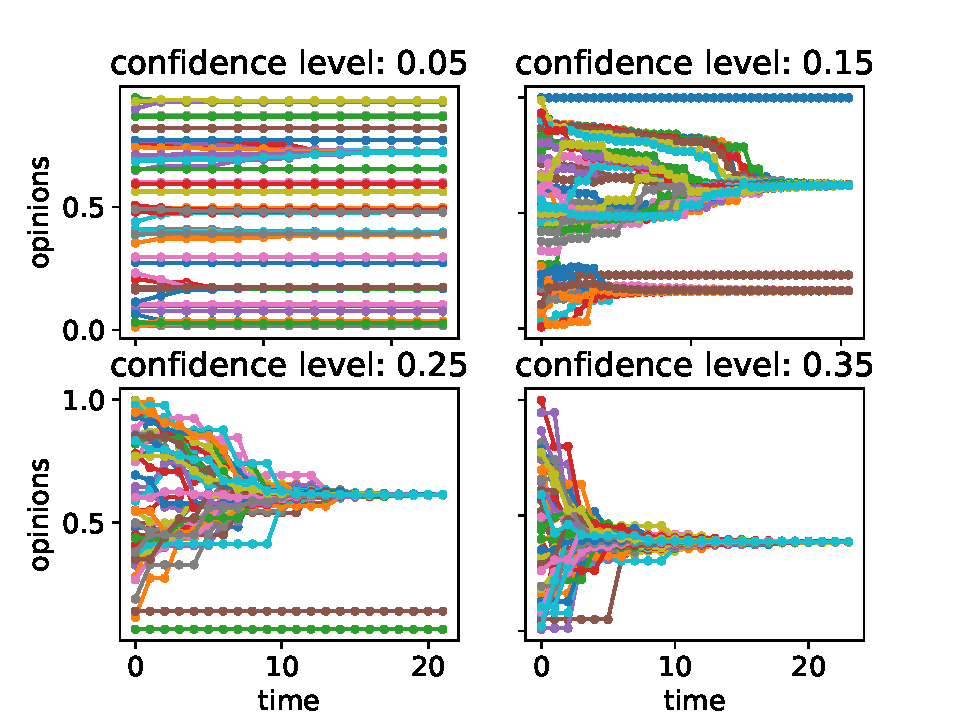
\includegraphics[width=\textwidth]{/home/arti/studia/python/praca_magisterska/plots/single_ws_50_10_0,3.pdf}
		\caption{Opinions dynamics for Watts--Strogatz network with $n=50$, $k=10$, $p=0.3$ and various confidence levels.}
		\label{f3}
\end{figure}
For Watts--Strogatz network (see Fig. \ref{f3}) we observe that for confidence level $\epsilon=0.05$ the simulation leaded to fragmentation of opinions, similarly as for complete graph network (see Fig. \ref{f2}). However, in Watts--Strogatz network agents often did not change their opinions at all, because they were not connected with agents with similar opinions. Hence, we can observe fragmentation into a lot of clusters at the end of simulation.
\indent

For confidence level $\epsilon=0.15$ evolution of opinions leaded to formation of 3 clusters. For confidence level $\epsilon=0.25$ most part of network reached consensus, excluding two agents who did not change their initial opinions at all, in fact their opinions were extreme ones (close to 0 or 1). Finally, when confidence level was big enough ($\epsilon=0.35$) all agents in the network decided to share one opinion.
\indent

For Watts--Strogatz networks relaxation times of opinions formation are longer than for a complete graph networks, agents change their opinions slowly.

\subsubsection{Barabasi--Albert}

\begin{figure}[H]
		\centering
		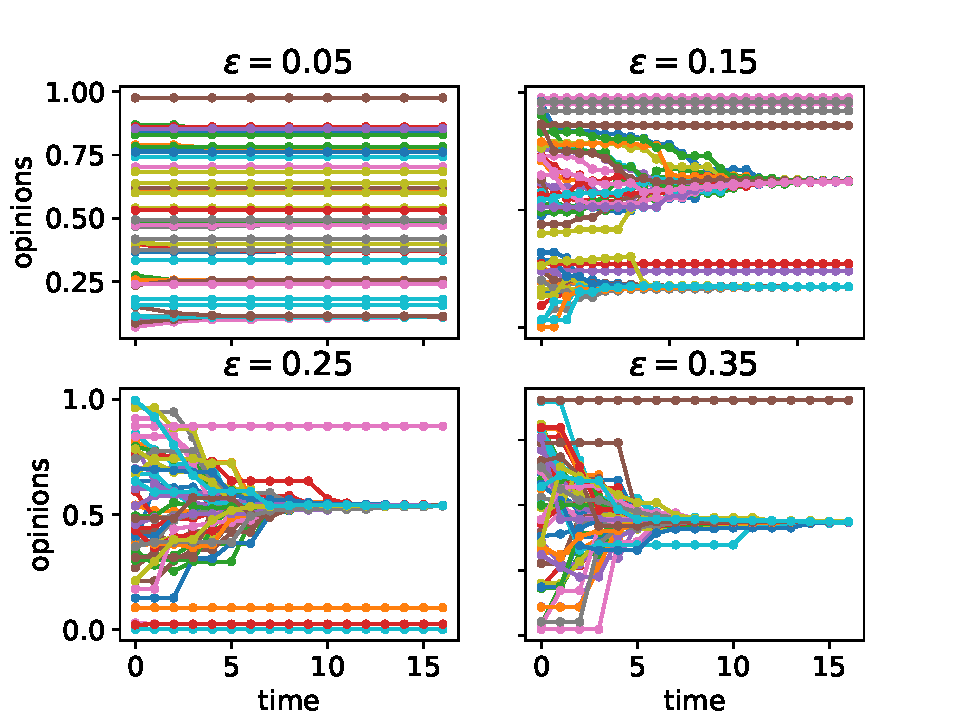
\includegraphics[width=\textwidth]{/home/arti/studia/python/praca_magisterska/plots/single_ba_50_4.pdf}
		\caption{Opinions dynamics for Barabasi--Albert network with $n=50$, $m=4$ and various confidence levels.}
		\label{f4}
\end{figure}
In the case of a Barabasi--Albert network we see that agents change their opinions mostly in the initial phase of the opinion dynamics (see Fig. \ref{f4}). 
\indent

For $\epsilon=0.05$ a lot of different opinions survived, similarly as for Watts--Strogatz network (see Fig. \ref{f3}). For $\epsilon=0.15$ we observe fragmentation into 3 clusters. One cluster (with opinion close to 0.5) is much bigger than the other two (with opinions close to 0.1 and 0.8). Beyond theses clusters, there are 3 agents, who did not change their opinions. Their opinions are extreme ones.
\indent

For $\epsilon=0.25$ we also observe that 3 clusters were formed. Moreover, again one cluster is significantly bigger than the others. There is one agent with opinion close to 1, who was not influenced by anybody. For $\epsilon=0.35$ most of the agents agreed on one common opinion, except one individual.


\subsection{Distribution of final opinions}

We will now investigate what is a typical distribution of opinions in a network depending on the value of the confidence level. We rounded final opinions of agents to two decimal places and calculated the average frequency of occurrences of rounded opinion values. We present the results on three--dimensional plots. First dimension represents the opinion space, second -- the confidence level and third one -- the opinion frequency.

\subsubsection{Complete graph}

\begin{figure}[H]
		\centering
		\includegraphics[width=0.7\textwidth]{/home/arti/studia/python/praca_magisterska/plots/avg_freq_cg_200_1.pdf}
		\caption{Distribution of final opinions for complete graph network with $n=200$ as a function of confidence level.}
		\label{f5}
\end{figure}

As can be seen in Fig. \ref{f5}, for complete graph we obtained results similar to those of Ref. \cite{bc}. The only difference is that we obtained positive frequency for some extreme opinion values even if most of the network typically reach consensus ($\epsilon > 0.25$). This is caused by a different updating schema used than in Ref. \cite{bc}. In our case there is a non--zero probability that an extreme opinion of some agent will be not influenced for some time and that in the same time other agents will change their opinions so strongly that they would have no chance to influence him later on. On the other hand, when sequential updating schema is applied to the model (used in Ref. \cite{bc}), then in one MCS all the agents change their opinions exactly once. As a result, surviving of extreme opinions is not common then.
\indent

Looking closer at the average frequency of final opinions for the complete graph, we can see that as the confidence level grows, the distribution of opinions is more centralized. For a very small confidence level ($\epsilon=0.01$) opinions are distributed uniformly on interval $(0, 1)$ (fragmentation). Situation changes for bigger values of the confidence level. When we look at $\epsilon=0.1$ we can observe similar distribution in the middle of opinion space ($0.25-0.75$) but extreme opinions (close to 0 or 1) do not emerge. Moreover, for opinion intervals ($0.1-0.25$) and ($0.75-0.9$) opinion frequency is higher. This phenomena of disappearance of extreme opinions and more frequent appearance of opinions in two regions which are symmetric with respect to the middle of opinions space continues to evolve up to confidence level $\epsilon=0.2$. We can also see that as we are closer to confidence level $\epsilon=0.2$, in the middle of opinions space ($0.35-0.65$) less opinions survive. This is a typical case of polarization of opinions. In the case of polarization typically one part of agents go for opinions around $0.25$ and the second part for opinions around $0.75$.
\indent

If we increase confidence level again to $\epsilon=0.25$ we can observe a phase transition from polarization of opinions to consensus. In the case of consensus, final opinions concentrate around the midpoint of the opinion space (i.e. the value $0.5$).


\subsubsection{Watts--Strogatz}

\begin{figure}[H]
		\centering
		\includegraphics[width=0.7\textwidth]{/home/arti/studia/python/praca_magisterska/plots/avg_freq_ws_200_6_0,2_1.pdf}
		\caption{Distribution of final opinions for Watts--Strogatz network with $n=200$, $k=6$, $p=0.2$ as a function of confidence level.}
		\label{f6}
\end{figure}

In Watts--Strogatz network with $k=6$ and $p=0.2$ we can see that the frequencies of opinions have different distribution than in the complete graph case (see Fig. \ref{f6}). For $\epsilon < 0.1$ we see uniform distribution on the whole opinions space. It is due to the fact that each agent have only 6 neighbors and not much confidence to them. Hence, agents do not change their initial opinions often. For confidence level $\epsilon=0.15$ distribution of opinions has 3 small peaks around opinions values: 0.25, 0.5, 0.75, beyond this peaks it is close to uniform with less frequent extreme opinions. Going further to $\epsilon=0.2$, we see that opinions emerge mainly in the $(0.4-0.6)$ interval (consensus establishes), while for complete graph $\epsilon=0.2$ led to two main spaces of opinions concentrating (polarization). For confidence levels $\epsilon>0.2$ opinions concentrate mainly around point 0.5. Still opinions close to boundaries survive, for $\epsilon=0.3$ there occur opinions smaller than $0.2$ or bigger than $0.8$, for $\epsilon=0.4$ agent may not change opinion if it is smaller than $0.1$ or bigger than $0.9$.

\subsubsection{Barabasi--Albert}

\begin{figure}[H]
		\centering
		\includegraphics[width=0.7\textwidth]{/home/arti/studia/python/praca_magisterska/plots/avg_freq_ba_200_6_1.pdf}
		\caption{Distribution of final opinions for Barabasi--Albert network with $n=200$, $m=6$ as a function of confidence level.}
		\label{f7}
\end{figure}

For Barabasi--Albert network with $m=6$ (Fig. \ref{f7}) extreme opinions survive for all values of the confidence level. Distribution's shape is rather more similar to complete graph case than to the Watts--Strogatz one. The polarization of opinions emerges for confidence levels around $\epsilon=0.15$. For $\epsilon=0.2$ the network starts to reach consensus more frequently -- we can see high peak in opinion frequency for values around 0.5. Up to $\epsilon=0.2$ we obtain positive opinion frequency in full range of opinions. Then, increasing the confidence level causes that single opinions might survive only if their are more extreme. Of course, the results may be different when network will have more connections (bigger value of parameter $m$). 

\subsection{Impact of the confidence level on reaching consensus}
We will investigate in this section which values of confidence level typically lead to consensus as the final state of opinion evolution process and how does the network size and network topology affect probability of reaching consensus. For each network topology we conducted simulations for various sets of parameters. We assumed that consensus was reached when 80\% of agents shared common opinion. For each value of the confidence level and a given network topology with its parameters, we simulate BC model 100 times and calculate probability of reaching consensus as the number of simulations that reached consensus divided by the total number of simulations. 

\begin{figure}[H]
		\centering
		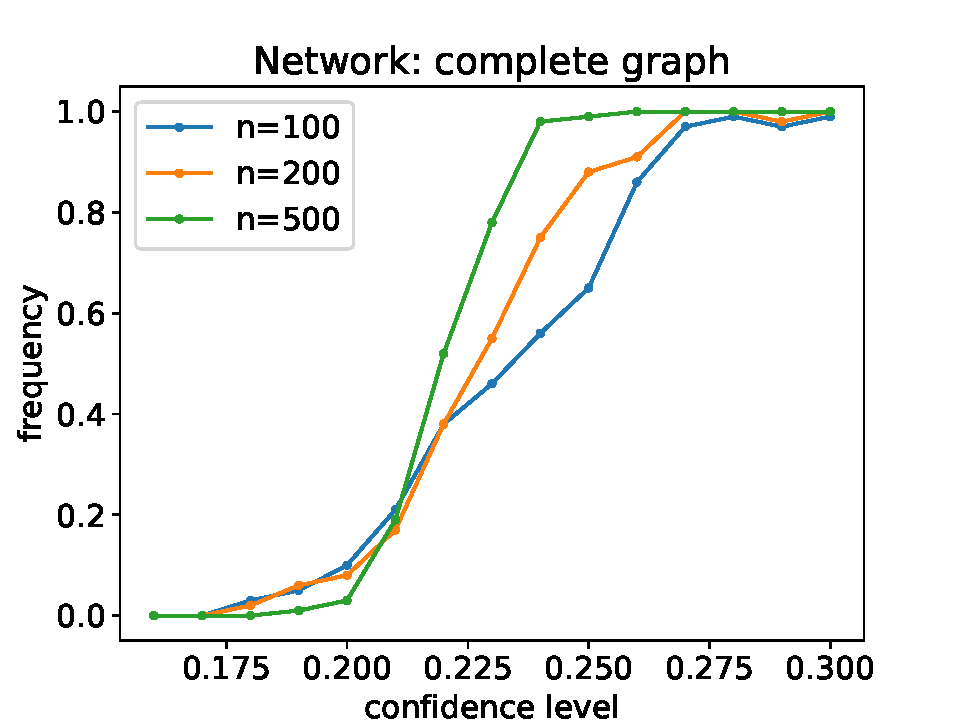
\includegraphics[width=0.7\textwidth]{/home/arti/studia/python/praca_magisterska/plots/freq_consensus_cg.pdf}
		\caption{Probability of reaching consensus for a complete graph network as a function of confidence level for various $n$.}
		\label{freq_cg}
\end{figure}

In Fig. \ref{freq_cg} the impact of network size on probability of reaching consensus for a complete graph topology is shown. For networks of sizes $n=100$, $n=200$ when confidence level $\epsilon\leq0.18$ we hardly ever reach consensus, while $\epsilon\geq0.27$ leads to reaching consensus almost every time.
For network size $n=500$ we hardly ever reach consensus when $\epsilon\leq0.2$ and almost every time reach consensus when $\epsilon\geq0.24$. The jump for probability of reaching consensus from 0 to 1 becomes more concentrated around one point when size of the network is bigger.  
We observe phase transition to reaching consensus, which is diluted by the finite size of the network.

\begin{figure}[H]
		\centering
		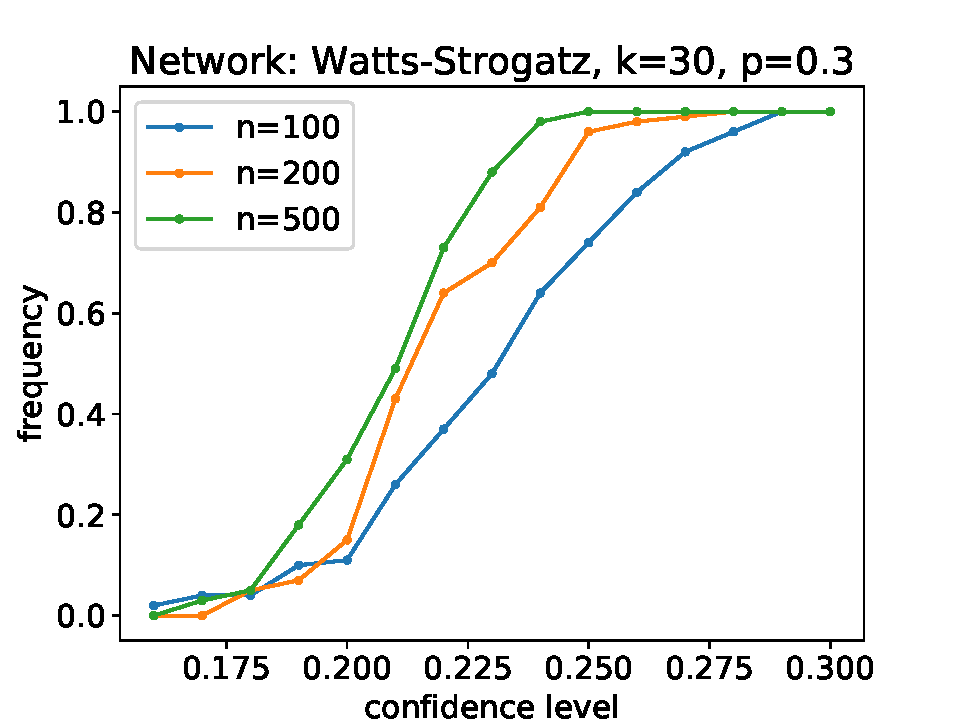
\includegraphics[width=0.7\textwidth]{/home/arti/studia/python/praca_magisterska/plots/freq_consensus_ws_k=30_p=0,3.pdf}
		\caption{Probability of reaching consensus for Watts--Strogatz network with $k=30$, $p=0.3$ as a function of confidence level for various $n$.}
		\label{f9}
\end{figure}

We can see in Fig. \ref{f9} that the bigger value of network size is, the closed the probability of reaching consensus to 1. For instance we reach consensus almost every time at confidence level:
\begin{itemize}
\item  $\epsilon=0.29$ for network size $n=100$,
\item  $\epsilon=0.26$ for network size $n=200$,
\item  $\epsilon=0.24$ for network size $n=500$.
\end{itemize}
\indent

We see that the bigger is the network, the more eager are agents to reach consensus (when $\epsilon>0.2$).

\indent

Next, we will check what influence on reaching consensus the parameter $k$ has. For that purpose we set network size $n=200$, parameter $p=0.3$ and conducted simulations of the model. Results are presented in Fig. \ref{freq_ws}.

\begin{figure}[H]
		\centering
		\includegraphics[width=0.7\textwidth]{/home/arti/studia/python/praca_magisterska/plots/freq_consensus_ws_200_p=0,2.pdf}
		\caption{Probability of reaching consensus for Watts--Strogatz network with $n=200$, $p=0.2$ as a function of confidence level for various $k$.}
		\label{freq_ws}
\end{figure}

We can see that with an increasing $k$, it is harder to reach consensus. It means that networks in which agents are well--connected are not so likely to agree on a one common opinion as weaker connected networks. For instance, we obtained consensus in almost 80\% of simulations for confidence level $\epsilon=0.2$ when $k=10$ and not even in 30\% of simulations for the same level when $k\geq20$.
\indent
Moreover, we see from Fig. \ref{freq_ws} that the higher the value of $k$, the closer the results to the complete graph (i.e. full connectance among agents). If an agent has initially $k=40$ neighbors, the results of the simulations are practically indistinguishable from the complete graph ones.

\indent

To better understand what $k$ values are typical for reaching consensus, we also plot probability of reaching consensus against $k$ in range $(4-20)$ for few values of confidence level.

\begin{figure}[H]
		\centering
		\includegraphics[width=0.7\textwidth]{/home/arti/studia/python/praca_magisterska/plots/eps_freq_consensus_ws_200_p=0,2.pdf}
		\caption{Probability of reaching consensus for Watts--Strogatz network with $n=200$, $p=0.2$ as a function of $k$ for various values of $\epsilon$.}
		\label{freq_ws_eps}
\end{figure}

It turns out that consensus is most likely to be reached when $k=6$ and $k=8$, which are cases of low number of connections. For $k=4$ agents are too weekly--connected and they can not influence each other so much, thus they agree on consensus rarely. For $\epsilon$ up to $0.22$ increasing $k$ starting from $k=8$ causes decreasing of probability of reaching consensus.

\indent

We already manipulated $n$ and $k$ parameters, now we will simulate model for different values of parameter $p$, setting $n=200$, $k=20$ (see Fig. \ref{f12}).

\begin{figure}[H]
		\centering
		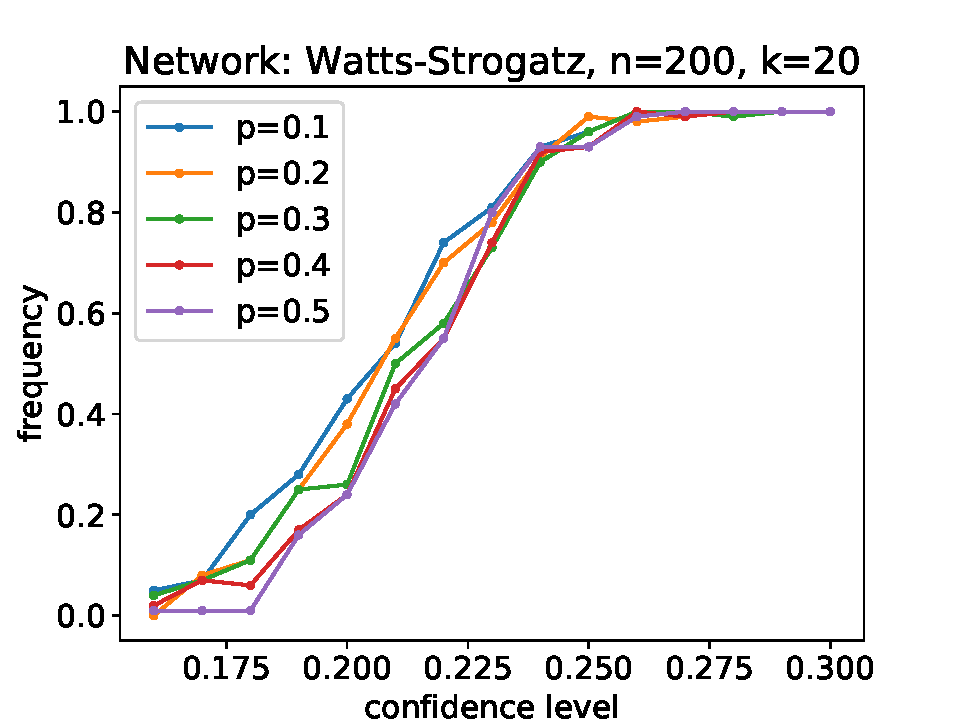
\includegraphics[width=0.7\textwidth]{/home/arti/studia/python/praca_magisterska/plots/freq_consensus_ws_200_k=20.pdf}
		\caption{Probability of reaching consensus for Watts--Strogatz network with $n=200$, $k=20$ as a function of confidence level for various values of $p$.}
		\label{f12}
\end{figure}

We see that with increasing $p$ the curves shift to the right, i.e. it is harder to reach consensus and higher confidence levels are needed to compensate the effects related to the rewiring of links.

Rewiring of links (parameter $p$) has no such a great impact on probability of reaching consensus as network connectivity (parameter $k$). Nevertheless, we observe significant increase in probability when we increase $p$ from $0.1$ to $0.5$.

\indent

For Barabasi--Albert networks we firstly set $m=6$ and manipulated network size $n$. Results are presented in Fig. \ref{f13}.

\begin{figure}[H]
		\centering
		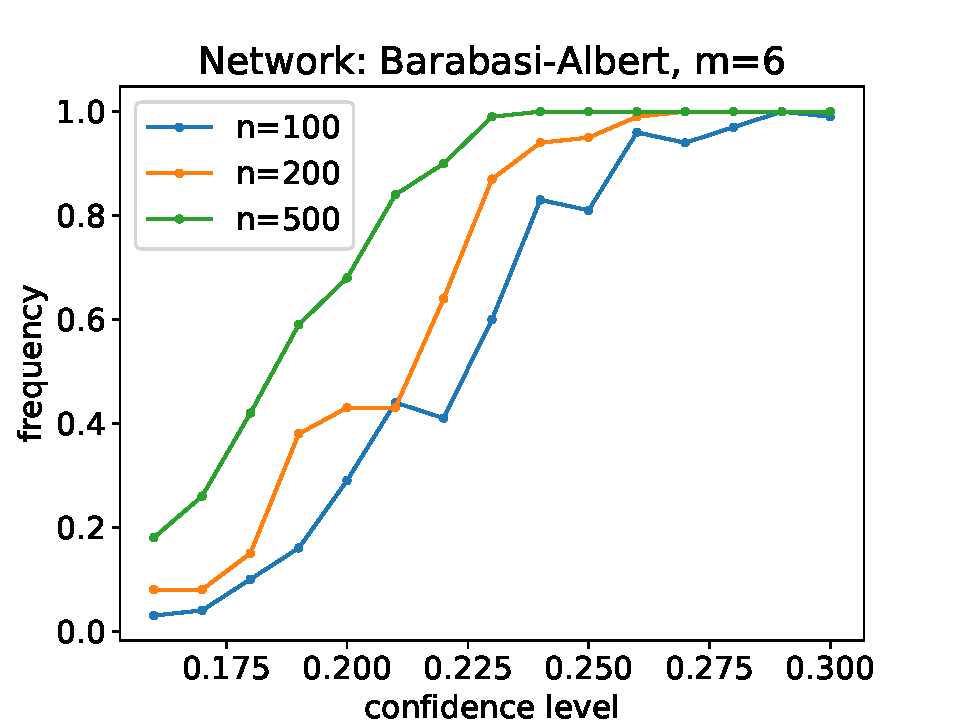
\includegraphics[width=0.7\textwidth]{/home/arti/studia/python/praca_magisterska/plots/freq_consensus_ba_m=6.pdf}
		\caption{Probability of reaching consensus for Barabasi--Albert network with $m=6$ as a function of confidence level for various values of $n$.}
		\label{f13}
\end{figure}

Similarly to the Watts--Strogatz case, increasing network size in Barabasi--Albert case is beneficial for reaching consensus at a given confidence level. Probability of reaching consensus is close to 1, when:
\begin{itemize}
\item  $\epsilon=0.29$ for network size $n=100$,
\item  $\epsilon=0.26$ for network size $n=200$,
\item  $\epsilon=0.22$ for network size $n=500$.
\end{itemize}

\indent

Next, we set $n=200$ and manipulated parameter $m$. Results are shown in Fig. \ref{freq_ba}.

\begin{figure}[H]
		\centering
		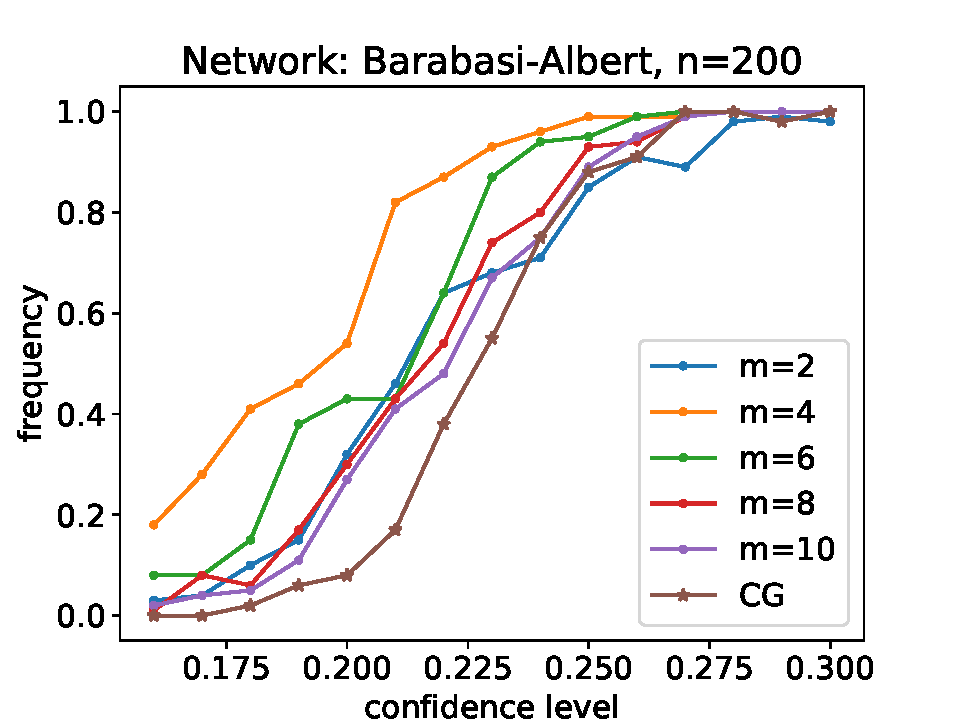
\includegraphics[width=0.7\textwidth]{/home/arti/studia/python/praca_magisterska/plots/freq_consensus_ba_200.pdf}
		\caption{Probability of reaching consensus for Barabasi--Albert network with $n=200$ as a function of confidence level for various values of $m$.}
		\label{freq_ba}
\end{figure}

We observe that for $m=4$ the probability of reaching   consensus is the highest. Increasing $m$ causes less frequent establishing of consensus. For $m=8$ and $m=10$ results are nearly the same, consensus is more likely than for complete graph, but differences in probability are not so big. Similarly to the Watts--Strogatz case, smaller number of connections affects higher chance for consensus. An exception from this rule is $m=2$. For $m=2$ network is weak--connected and as a result probability of reaching consensus is not so big as for $m=4$ or $m=6$.

\subsection{Dynamics of opinions changing}
In this section we will study average changes of agents opinions in the course of time. We will investigate what is average change of opinions depending on confidence level, we will calculate the average opinion change by the following formula:
\begin{equation}
\Delta x = \frac{ \sum_{i=1}^n \left|x_{f}^{(i)} - x_0^{(i)} \right|}{n},
\end{equation}
where $x_0^{(i)}$ and $x_{f}^{(i)}$ are the initial and the final opinions of the i-th agent respectively.

\indent

We will also study what is the dynamics of opinions changes depending on given network. In order to do this after each MCS of BC model simulation, we calculate average value of opinion change, that is:
\begin{equation}
\Delta x_t = \frac{\sum_{i=1}^n \left|x_{t+1}^{(i)} - x_{t}^{(i)} \right|}{n}.
\end{equation}

Results for complete graph are shown in Fig. \ref{f15}.

\begin{figure}[H]
		\centering
		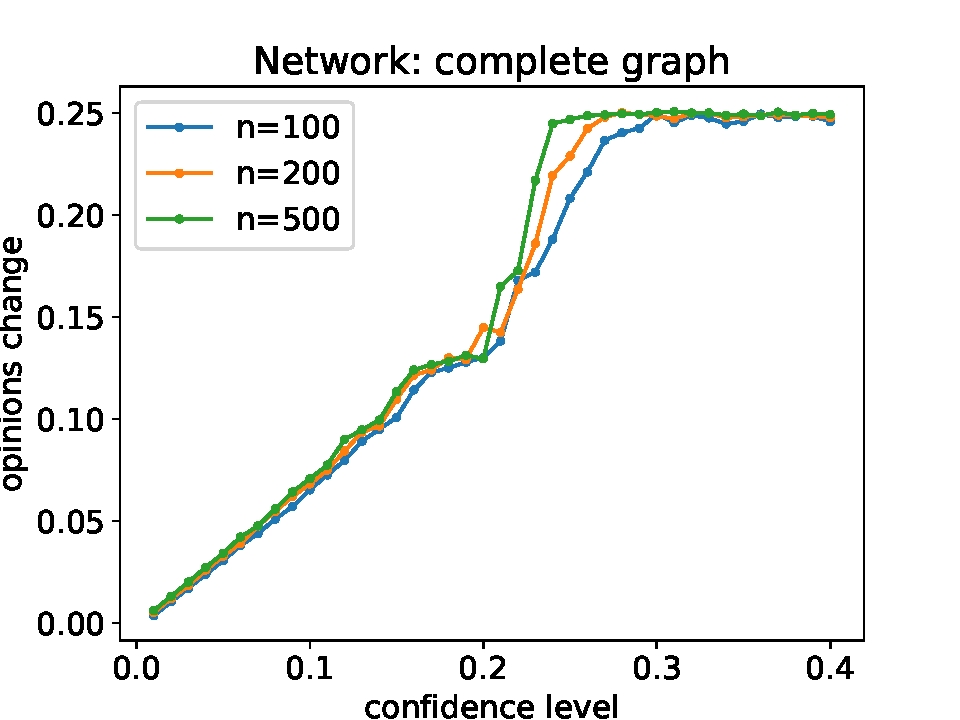
\includegraphics[width=0.7\textwidth]{/home/arti/studia/python/praca_magisterska/plots/changes_completegraph.pdf}
		\caption{Average change of opinion for complete graph as a function of confidence level for various values of $n$.}
		\label{f15}
\end{figure}

We see that the average agents opinions change increases with the confidence level $\epsilon$. We observe linear growth up to $\epsilon=0.17$, at this point value of the opinion change is around $0.13$. Further on, up to $\epsilon=0.2$ the change increases only slightly due to the phase transition from fragmentation to polarization. To this point plots for different network sizes are similar. We may claim that $\epsilon=0.2$ is a critical point, because in its vicinity a small increase of the confidence level causes significant changes of opinions. Although the curves for different system sizes are similar, we observe that the steepest growth is for biggest network ($n=500$) and the smallest growth is for $n=100$. Finally, opinion changes stabilize on value $0.25$, which is typical case of consensus.

\indent

We already know how confidence level affects differences between initial agents opinions and final, but we would also like to know what is the dynamics of opinions changes. The corresponding plots are shown in Fig. \ref{f16}.

\begin{figure}[H]
		\centering
		\includegraphics[width=\textwidth]{/home/arti/studia/python/praca_magisterska/plots/steps_changes_completegraph.pdf}
		\caption{Average change of opinion as a function of time for complete graph network for various values of $\epsilon$ and $n$.}
		\label{f16}
\end{figure}

We observe the biggest changes in opinion dynamics in first 3 MCS of simulation. The values of changes are bigger for bigger $\epsilon$. Opinion changing decrease with the course of time and after just a few MCS it disappears. An exception is $\epsilon=0.25$. For this confidence level, the system sometimes initially polarizes but then transforms to consensus (see $\epsilon=0.25$ in Fig. \ref{f2}). In these situations a lot of opinion changing takes place when $t>10$. Hence, we see small after averaging opinion changing for $t>10$.

\indent

For Watts--Strogatz network we compare opinion changes depending on $k$ parameter. We consider networks with low number of connections ($k$ in range $4-12$), as well as well--connected networks ($k$ in range $10-50$).

\begin{figure}[H]
		\centering
		\includegraphics[width=0.7\textwidth]{/home/arti/studia/python/praca_magisterska/plots/pairs_changes_ws.pdf}
		\caption{Average change of opinion for Watts--Strogatz network with $n=200$, $p=0.2$ as a function of confidence level for various values of $k$.}
		\label{f17}
\end{figure}

From the plots shown in Fig. \ref{f17} it follows that there are single curves which differs the most from the rest, for the frist plot it is $k=4$ and for the second it is $k=10$. 
\indent

In the first case, $k=4$ means that agents have too less connections with neighbors to change their opinions significantly, small number of potential influential neighbors causes agents to stick with their own opinion if none of neighbors has similar point of view. If we increase $k$ to $6$, then chances of finding someone influential increase by 50\% and that is the reason why agents change their opinions more in that case. For $k$ from $6$ to $12$ we observe that more connections means larger opinions changes if $\epsilon < 0.15$. For $0.15 \leq \epsilon \leq 0.20$ obtained results are similar and then for $\epsilon > 0.20$ we see a little bigger opinions changes for bigger $k$. It might look strange that for $k=6$ we have smaller average opinions change than for $k=8, 10, 12$ when $0.2 \leq \epsilon \leq 0.25$, whereas it was shown that for $k=6$ agents are more eager to agree on consensus on considered confidence levels (see Figure \ref{freq_ws_eps}). It happens so, because even when most part of network decide to share the same opinion (at least 80\% of network), there are still some agents (especially for small $k$), who stick to their own opinions, which causes lowering of average opinions change.
\indent

On the second plot we see that opinions changes for $k=10$ are the smallest ones when $\epsilon \leq 0.08$ and the biggest ones when $0.11 \leq \epsilon \leq 0.23$. For small confidence level, e.g. $\epsilon=0.05$ and for $k=10$ probability that at least one neighbor of given agent will have similar opinion is small and that is why agents do not change their opinions much, while for $k=20$ this probability is bigger and agents change their opinions more. For $\epsilon$ around $0.2$ we obtain bigger opinions changes for $k=10$, it is the case when consensus is reached more often for that value of $k$ than for $k=20$ or bigger (see Figure \ref{freq_ws}). We can also notice that starting from $k=20$ we obtain similar results in comparison to complete graph (linear growth up to $\epsilon=0.15$, steep growth from $\epsilon=0.20$ to $\epsilon=0.25$ and average opinion change around level $0.25$ for $\epsilon>0.25$).

\indent

Knowing how final opinions differ from initial ones, we can now analyze the dynamics of opinion changes (Fig. \ref{f18}).

\begin{figure}[H]
		\centering
		\includegraphics[width=\textwidth]{/home/arti/studia/python/praca_magisterska/plots/steps_changes_Watts-Strogatz_n=200_p=0_2.pdf}
		\caption{Average change of opinion as a function of time for Watts--Strogatz network with $n=200$, $p=0.2$ for various values of $\epsilon$ and $k$ ranging from $4$ to $12$.}
		\label{f18}
\end{figure}

For $k$ from $4$ to $12$ we see that opinions changes are the biggest at the beginning and then they slowly decrease for further time steps. Also, it is common for all confidence levels that for $k=12$ agents change their opinions the most and for $k=4$ the least up to some moment in time. For $\epsilon=0.05$ not much happens, opinions changes are very small and network stabilizes quickly. For $\epsilon=0.15$ and $k \geq 0.06$ we see that agents change their opinions very slowly. When agent decide to change his opinion a bit, it may happen that he will then start to be influenced by another agent for whom he had no confidence earlier, the changed opinions might influence another agents and due to non--centralized topology of Watts--Strogatz network it takes a long time of slowly opinions changing to finally achieve stable state.
\indent

For $\epsilon=0.25$ we observe that the dynamics of opinions changing last the longest when $k=4$, for $\epsilon=0.35$ we obtain faster stabilizing due to higher confidence level.

\begin{figure}[H]
		\centering
		\includegraphics[width=\textwidth]{/home/arti/studia/python/praca_magisterska/plots/steps_changes_Watts-Strogatz_n=200_p=0_2_1.pdf}
		\caption{Average change of opinion as a function of time for Watts--Strogatz network with $n=200$, $p=0.2$ for various values of $\epsilon$ and $k$ ranging from $10$ to $50$.}
		\label{f19}
\end{figure}

In Fig. \ref{f19} same plots for even higher values of $k$ are shown. All plots for $k \geq 20$ look similar to each other, again biggest changes in opinions dynamics can be observed at the beginning of the process. At confidence level $\epsilon=0.05$ for $k \geq 20$ opinions does not stabilize so quickly as in case of $k=10$. When $\epsilon=0.15$ we see opposite situation, for $k=10$ opinions changes decrease very slowly. When $\epsilon=0.25$ we observe slow disappearing of opinion changing, this behavior could be caused by slow transformation from polarization of opinions to consensus, network firstly polarize to two main clusters, but then agents decide to accept one common opinion. When $\epsilon=0.35$ consensus is reached quicker, system stabilize after few steps.

\indent

We would also like to check what influence on opinions change does $p$ parameter has (Fig. \ref{f20}).

\begin{figure}[H]
		\centering
		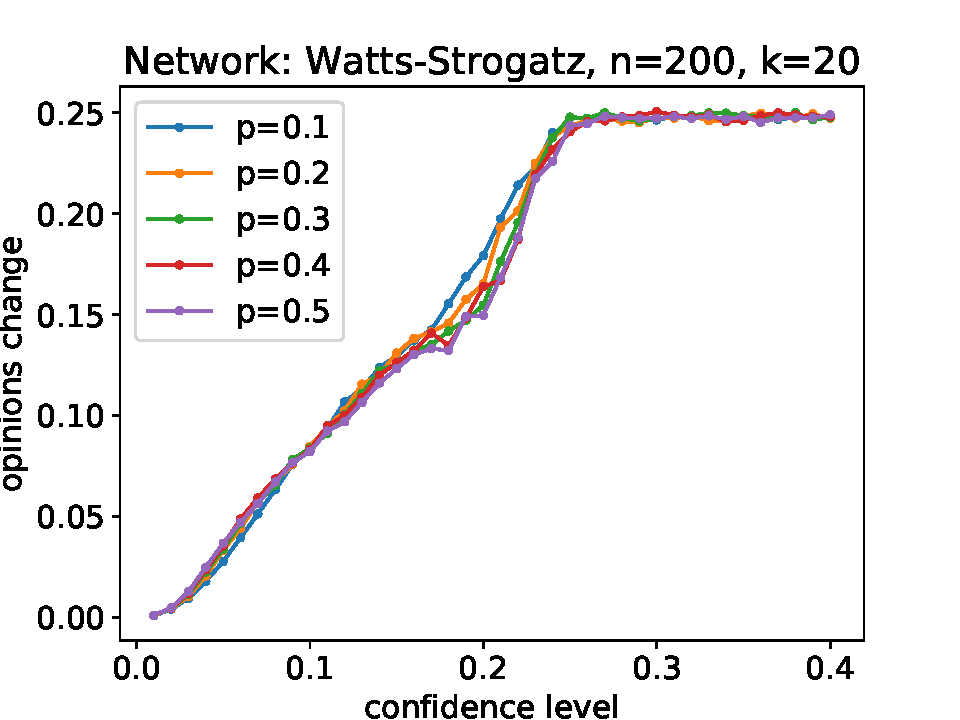
\includegraphics[width=0.7\textwidth]{/home/arti/studia/python/praca_magisterska/plots/changes_Watts-Strogatz_n=200_k=20.pdf}
		\caption{Average change of opinion for Watts--Strogatz network with $n=200$, $k=20$ as a function of confidence level for various values of $p$.}
		\label{f20}
\end{figure}

Results for changes of opinions are similar for various values of parameter $p$. However, there are noticeable differences in region $0.15 \leq \epsilon \leq 0.25$. In that region agents in networks with smaller value of $p$ tend to change their opinions more likely, regular connections in network promote opinion changing more than random ones.

\indent

Now we will look on the dynamics of changing opinions for networks with various $p$ (Fig. \ref{f21}).


\begin{figure}[H]
		\centering
		\includegraphics[width=\textwidth]{/home/arti/studia/python/praca_magisterska/plots/steps_changes_Watts-Strogatz_n=200_k=20.pdf}
		\caption{Average change of opinion as a function of time for Watts--Strogatz network with $n=200$, $k=20$ for various values of $\epsilon$ and $p$.}
		\label{f21}
\end{figure}

When $\epsilon=0.05$ agents in network with $p=0.5$ change opinions the slowest and in network with $p=0.1$ the fastest. The opposite results are for $\epsilon \geq 0.15$. The bigger is $p$, the more random is the structure of the network. It also implies shorter paths between agents and therefore opinion changing is less time consuming when $p=0.5$.

\indent

Let's now look how final opinions differ from initial for Barabasi--Albert network (Fig. \ref{f22}).

\begin{figure}[H]
		\centering
		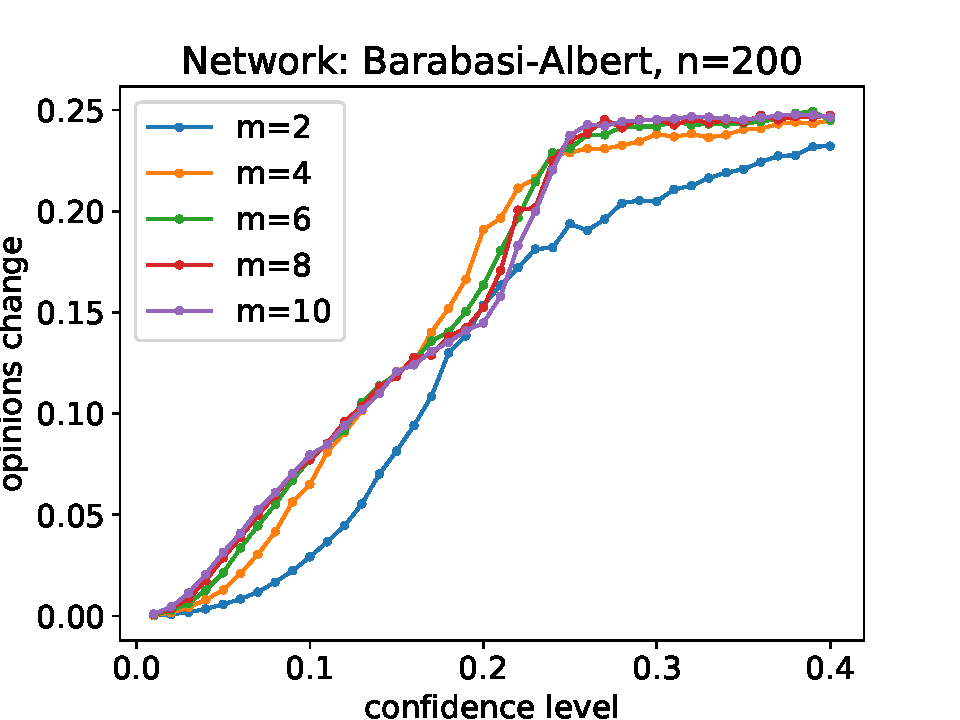
\includegraphics[width=0.7\textwidth]{/home/arti/studia/python/praca_magisterska/plots/changes_Barabasi-Albert_n=200.pdf}
		\caption{Average change of opinion for Barabasi--Albert network with $n=200$ as a function of confidence level for various values of $m$.}
		\label{f22}
\end{figure}

We can see that for $m=2$ opinions changes are smaller than for bigger values of $m$, which is caused by too sparse connections in the network. For the other values of $m$ the curves have similar shape. Firstly, there is almost linear growth in opinion changing up to $\epsilon=0.2$. Then, there is a steeper growth up to $\epsilon=0.25$. From this $\epsilon$ opinion change stabilizes on value $0.25$. The results for Barabasi--Albert networks are similar to complete graph case.

\begin{figure}[H]
		\centering
		\includegraphics[width=\textwidth]{/home/arti/studia/python/praca_magisterska/plots/steps_changes_Barabasi-Albert_n=200.pdf}
		\caption{Average change of opinion as a function of time for Barabasi--Albert network with $n=200$ for various values of $\epsilon$ and $m$.}
		\label{acba}
\end{figure}

In Fig. \ref{acba} the dynamics of opinion change is presented. Similarly to complete graph and Watts--Strogatz networks, for BA networks opinion changes are the biggest at the beginning of the time evolution. The bigger is the value of $m$, the bigger are the changes in first few time steps. When $\epsilon=0.15$ we observe the longest opinion changing for $m=4$, whereas $\epsilon=0.15$ or $\epsilon=0.25$ leads to the longest opinion changing for $m=2$.

\indent

We conclude this chapter with a direct comparison of the results obtained for different networks (Fig. \ref{f24}).

\begin{figure}[H]
		\centering
		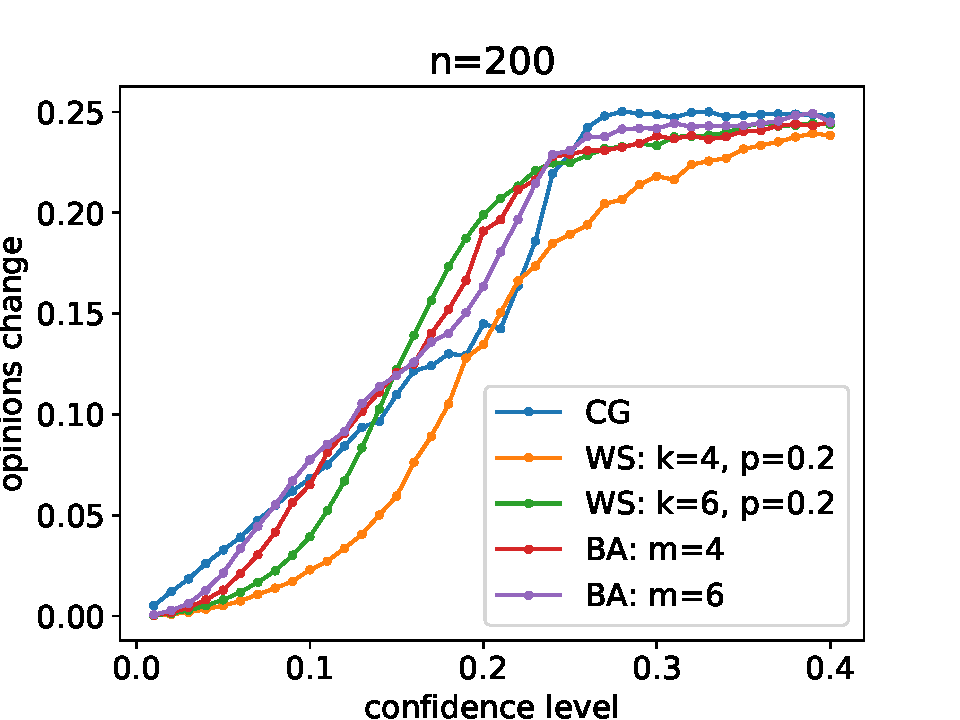
\includegraphics[width=0.7\textwidth]{/home/arti/studia/python/praca_magisterska/plots/changes_various.pdf}
		\caption{Average change of opinion for various networks with $n=200$ as a function of confidence level.}
		\label{f24}
\end{figure}

For small confidence level ($\epsilon \leq 0.05$) WS networks with $k=4,6$ and BA networks with $m=4,6$ are less opinion--changing than CG network. There is small number of links between agents in these networks, hence they are often not influenced when $\epsilon$ is small.
\indent

The less opinion changing network is WS with $k=4$. It is the most weak--connected one. Other networks have similar characteristics of opinion changing, differences between the curves are small.

\begin{figure}[H]
		\centering
		\includegraphics[width=\textwidth]{/home/arti/studia/python/praca_magisterska/plots/steps_changes_various.pdf}
		\caption{Average change of opinion as a function of time for various networks with $n=200$ and various $\epsilon$.}
		\label{f25}
\end{figure}

As it follows from Fig. \ref{f25}, the complete graph  has slightly different dynamics of changing opinions than other networks. In this case agents change opinions the most in first $2-4$ MCS of simulation and typically after just a few MCS system reach the stable state. In BA network this process is more stretched in time (excluding $\epsilon=0.05$ when not much happen for weak--connected networks). 
The longest process of small opinion changing occurs in WS networks due to long paths between agents.


\subsection{Fragmentation of opinions}

In this section we will study the issue of how many clusters are formed at the end of the process of opinions evolution (network fragmentation). In order to do this, we calculate average number of clusters, meaning connected components of the network. We take into account only these network connections for which absolute value of difference between agents final opinions is smaller or equal to confidence level. We are interested only in clusters, which have significant size. So, when we count how many clusters are formed, we skip clusters which have size smaller than $10\%$ of the size of the biggest cluster.

\indent

We will start with complete graph. The results are shown in Fig. \ref{f26}.

\begin{figure}[H]
		\centering
		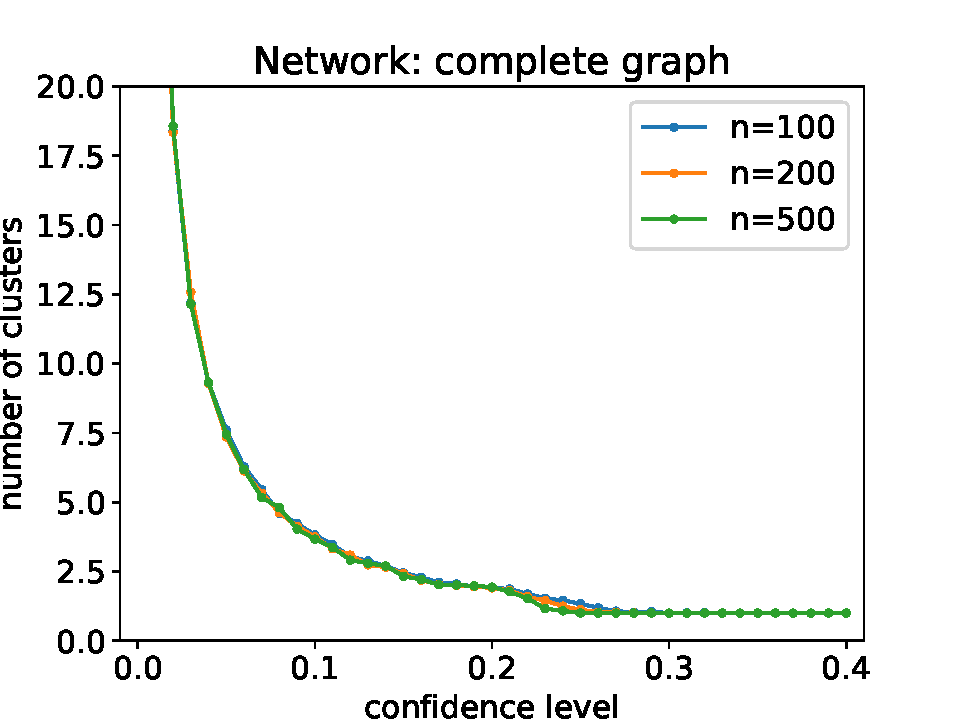
\includegraphics[width=0.7\textwidth]{/home/arti/studia/python/praca_magisterska/plots/groups10_completegraph.pdf}
		\caption{Average number of clusters for complete graph network as a function of confidence level for various values of $n$.}
		\label{f26}
\end{figure}

We observe that number of clusters in CG decreases when confidence level increases. For different network sizes results are very similar. We can distinguish few interesting cases:
\begin{itemize}
\item for small confidence level, e.g. $\epsilon = 0.05$, network typically partitions into few clusters having different opinions,
\item for confidence level $0.17 \leq \epsilon \leq 0.21$ network divides into two clusters (polarization of opinions),
\item for confidence level from $\epsilon = 0.22$ to $\epsilon = 0.26$ average number of clusters changes from $2$ to 	$1$, which corresponds to the transition from polarization of opinions to consensus, additionally we see that this transition is more rapid for larger networks ($n=500$),
\item for $\epsilon \geq 0.27$ average number of clusters is equal to $1$ (consensus).
\end{itemize} 

\indent

As far as the Watts--Strogatz network are concerned, in Fig. \ref{f27} the number of clusters as a function of $\epsilon$ for different values of $k$ is shown.

\begin{figure}[H]
		\centering
		\includegraphics[width=0.7\textwidth]{/home/arti/studia/python/praca_magisterska/plots/pairs_groups10_ws.pdf}
		\caption{Average number of clusters for Watts--Strogatz network with $n=200$, $p=0.2$ as a function of confidence level for various values of $k$.}
		\label{f27}
\end{figure}

We see that for small $k$ (top plot in Fig. \ref{f27}) the results strongly depend on its particular value. The higher $k$, the faster the number of clusters decreases. For instance, average number of clusters is around $6$ when:

\begin{itemize}
\item $\epsilon=0.16$ for $k=4$,
\item $\epsilon=0.11$ for $k=6$,
\item $\epsilon=0.09$ for $k=8$,
\item $\epsilon=0.08$ for $k=10$,
\item $\epsilon=0.07$ for $k=12$.
\end{itemize}

When $\epsilon=0.15$ there are 2 clusters in the average (polarization) for $k \geq 6$, whereas there are 10 clusters for $k=4$. Going further up to $\epsilon=0.23$ number of clusters decreases from $2$ to $1$. For $k=6,8$ this decreasing is the fastest, for $k=10,12$ a little bit slower and for $k=4$ definitely the slowest.

\indent
Comparing the case of $k=10$ to cases $k=20,30,40,50$ (bottom plot in Fig. \ref{f27}) we notice that for small confidence level up to $\epsilon=0.07$ average number of clusters is much bigger for $k=10$. On the other hand, when $\epsilon \geq 0.10$ average number of clusters is a little bit smaller for $k=10$ than for $k \geq 20$. Results for $k \geq 20$ are similar to each other and also to CG case.

\indent

It is also interesting to look at the impact of the rewiring probability $p$ (Fig. \ref{f28}).

\begin{figure}[H]
		\centering
		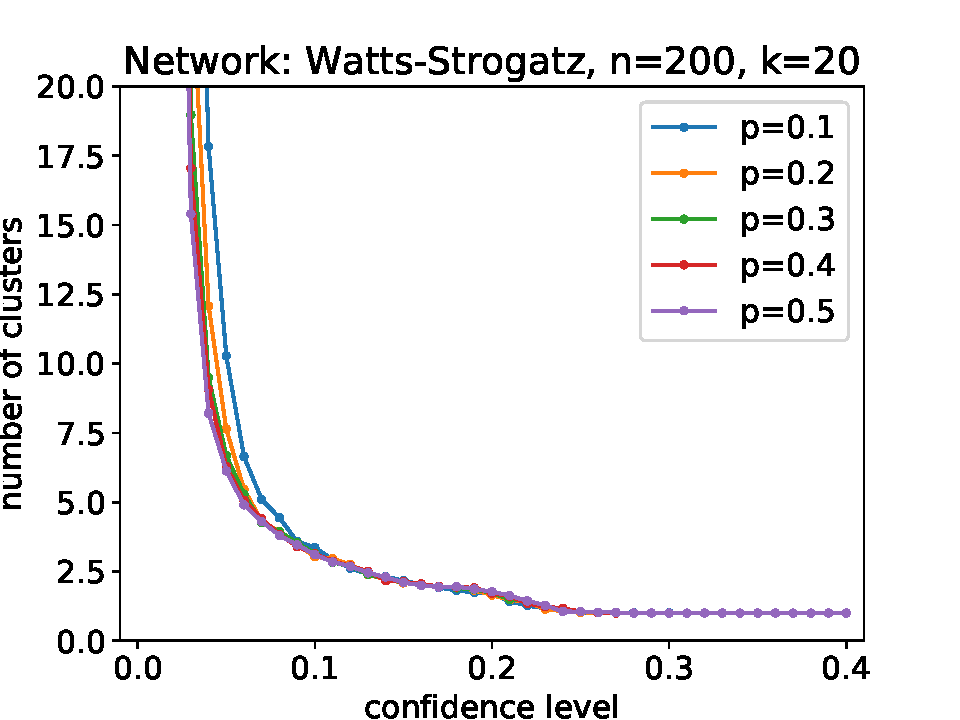
\includegraphics[width=0.7\textwidth]{/home/arti/studia/python/praca_magisterska/plots/groups10_Watts-Strogatz_n=200_k=20.pdf}
		\caption{Average number of clusters for Watts--Strogatz network with $n=200$, $k=20$ as a function of confidence level for various values of $p$.}
		\label{f28}
\end{figure}

We see that changing $p$ has practically no impact on the number of formed clusters. Results are pretty similar for all values of $p$. Only for small confidence levels (e.g. $\epsilon=0.05$) slightly more clusters form when $p$ is smaller.

\indent

The number of clusters as a function of $\epsilon$ for Barabasi--Albert networks with different values of the parameter $m$ is shown in Fig. \ref{f29}.

\begin{figure}[H]
		\centering
		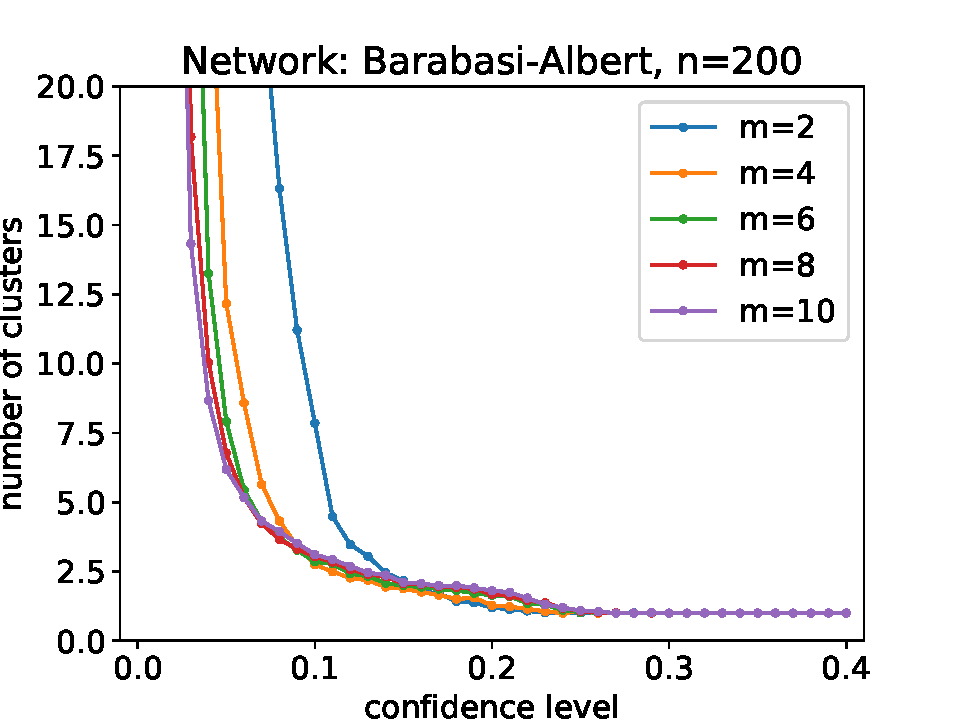
\includegraphics[width=0.7\textwidth]{/home/arti/studia/python/praca_magisterska/plots/groups10_Barabasi-Albert_n=200.pdf}
		\caption{Average number of clusters for Barabasi--Albert network with $n=200$ as a function of confidence level for various values of $m$.}
		\label{f29}
\end{figure}

We obtain similar results for average number of clusters as a function of $\epsilon$ for networks with $m=6,8,10$. When $\epsilon=0.07$ a bit more than 4 clusters are formed in these cases. It is 1 cluster less than in CG case. This difference decreases with $\epsilon$. When $\epsilon=0.15$, there are 2 clusters in the average for BA networks and 0.5 more fore CG. For higher $\epsilon$ results for $m \geq 6$ and CG are similar.

Looking on the plots for BA networks with $m=2$ and $m=4$ we see that they fragment into more clusters than networks with greater number of connections ($m \geq 6$) when confidence level is small (e.g. $\epsilon=0.05$). On the other hand, average number of clusters is the lowest for these networks when $\epsilon \geq 0.16$, they seem to prefer consensus over polarization more frequently than other networks.

\indent
When we investigated probability of reaching consensus, it turned out that networks with $m=4$ were likely to reach consensus, but with $m=2$ not so. Taking that into account, it might seem strange that $m=2$ led to the smallest average number of clusters (closest to $1$) when $\epsilon$ is around $0.2$. As the matter of fact, for $m=2$ there are many agents sharing one opinion, but also many agents are not influenced at all. When we were studying establishing consensus, we required at least $80\%$ of the network to share a common opinion. For $m=2$ one cluster often does not cover $80\%$ of the network due to many individuals sticking to their own opinion.

\indent

We will also compare various networks on one figure to see if the fragmentation of opinions differs between them (Fig. \ref{f30}).

\begin{figure}[H]
		\centering
		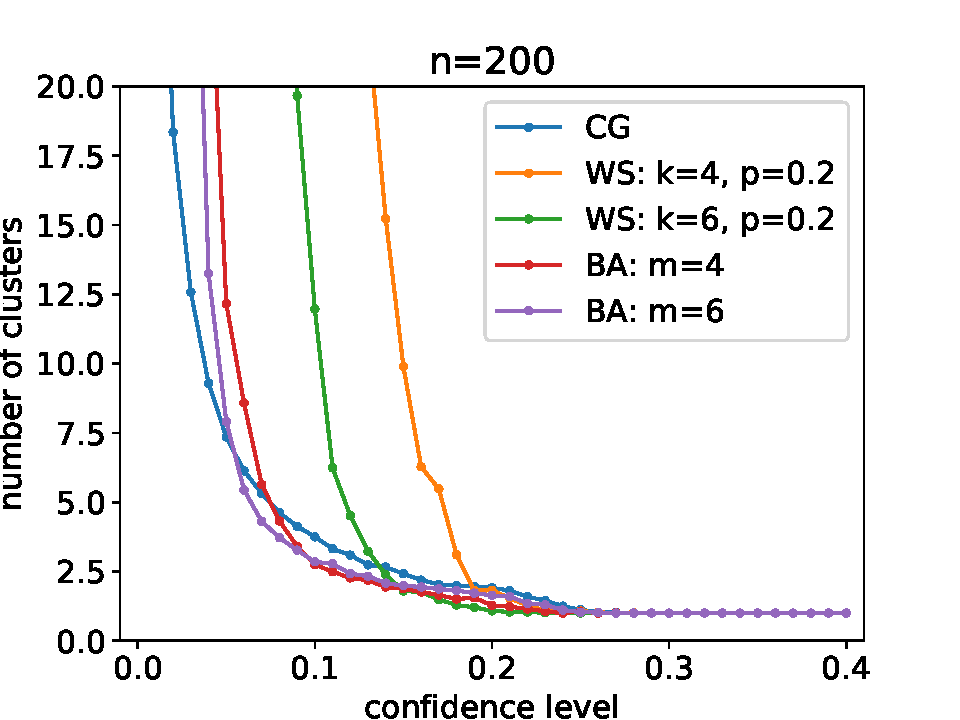
\includegraphics[width=0.7\textwidth]{/home/arti/studia/python/praca_magisterska/plots/groups10_various.pdf}
		\caption{Average number of clusters for various networks with $n=200$ as a function of confidence level.}
		\label{f30}
\end{figure}

We see that CG and BA networks have similar characteristics -- the number of clusters decreases quickly with $\epsilon$ for values of the confidence level smaller than $0.13$. In this regime fragmentation in WS networks is much higher. It is due to the fact that in WS networks all the agents have similar number of neighbors ($k$ in the average). There are no hubs who could convince others and concentrate clusters around themselves like in BA networks. 
\indent

For $0.13<\epsilon<0.18$ the more connected WS network ($k=6$) becomes similar to BA and CG. The less connected one is still more fragmented than the others.
\indent

For $\epsilon>0.18$ we observe only small differences between networks. The more connected WS network has the lowest average number of clusters, as its topology favors establishing consensus. Above $\epsilon=0.25$ all of networks are not fragmented anymore.


\subsection{Relaxation times}
In the studies of opinion dynamics in agent--based models, relaxation time can be defined as the time needed for the network to reach the stable state. In simulations of the BC model, we assume that system is relaxed when none of the agents changes his opinion by more than $0.001$ in one MCS. In this section we will check what is the relaxation time $t$ of opinions evolution process depending on confidence level for various network topologies.

\indent

Frist, we compare relaxation times for complete graph networks with various sizes (Fig. \ref{f31}).

\begin{figure}[H]
		\centering
		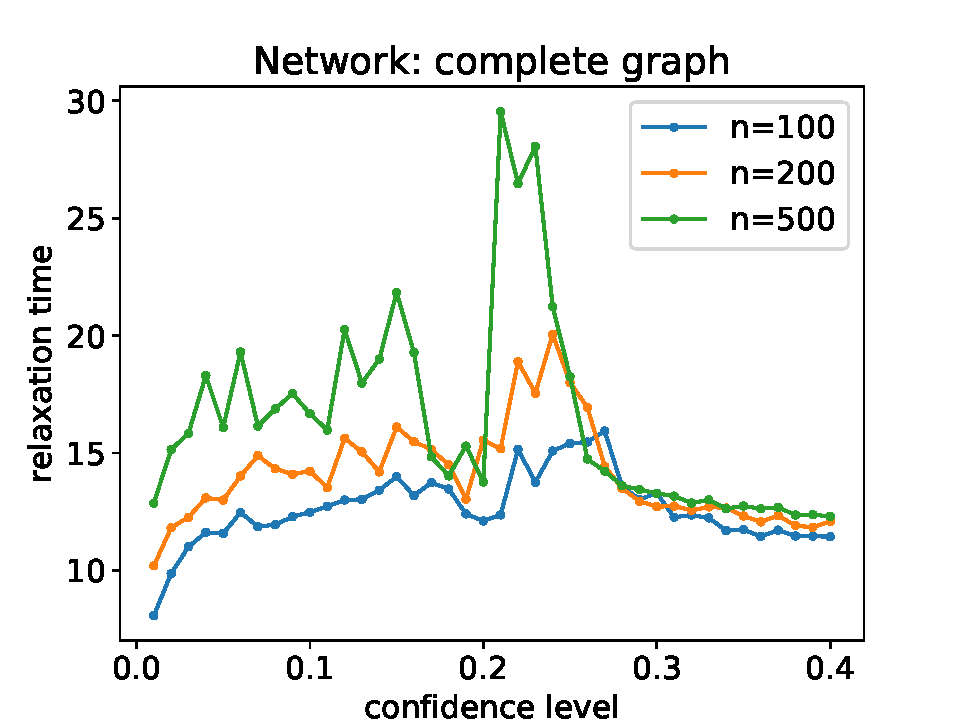
\includegraphics[width=0.7\textwidth]{/home/arti/studia/python/praca_magisterska/plots/steps_completegraph.pdf}
		\caption{Average relaxation time for complete graph network as a function of confidence level for various values of $n$.}
		\label{f31}
\end{figure}

We see that the bigger the size of a network is, the longer the relaxation time, especially for confidence levels up to $\epsilon=0.24$. We see smaller differences between results for various sizes when $\epsilon > 0.27$, in this case relaxation time is between $11$ and $13$ (MCS). 
\indent

For confidence level up to $\epsilon=0.15$ average relaxation time slowly increases for all sizes and also has not small variance (especially for $n=500$). Typical values of relaxation time for $\epsilon=0.1$ are:
\begin{itemize}
\item $t=12$ for $n=100$,
\item $t=14$ for $n=200$,
\item $t=17$ for $n=500$.
\end{itemize}
We observe also a critical slowing down (peaks in the relaxation times) for $0.20<\epsilon<0.27$, indicating the phase transition of the system from polarization to consensus (see Figure \ref{freq_cg}). We observe following peak values:
\begin{itemize}
\item $t=15$ for $n=100$,
\item $t=18$ for $n=200$, 
\item $t=27$ for $n=500$.
\end{itemize}

\indent

Results for Watts--Strogatz networks with different values of $k$ are shown in Fig. \ref{f32}.

\begin{figure}[H]
		\centering
		\includegraphics[width=0.7\textwidth]{/home/arti/studia/python/praca_magisterska/plots/pairs_steps_ws.pdf}
		\caption{Average relaxation time for Watts--Strogatz network with $n=200$, $p=0.2$ as a function of confidence level for various values of $k$.}
		\label{f32}
\end{figure}

For $k$ from $4$ to $12$ (top plot in Fig. \ref{f32}) we see common results for average relaxation time depending on confidence level. Relaxation time increases with $\epsilon$ up to some level, and after that it decreases. We also notice that for smaller $k$ peaks of relaxation times are bigger. Generally networks with smaller $k$ parameter relax faster for $\epsilon \leq 0.07$ but slower for $\epsilon \geq 0.18$. Peak values of relaxation times are around:
\begin{itemize}
\item $t=160$ for $k=4$ when $\epsilon=0.19$,
\item $t=160$ for $k=6$ when $\epsilon=0.16$,
\item $t=130$ for $k=8$ when $\epsilon=0.12$,
\item $t=120$ for $k=10$ when $\epsilon=0.11$,
\item $t=100$ for $k=12$ when $\epsilon=0.09$.
\end{itemize} 

When we consider $k=10, 20, 30, 40, 50$ (see bottom plot in Fig. \ref{f32}), we can observe much more faster relaxation of networks with $k \geq 20$ when $\epsilon \geq 0.10$, in this situation more connections in network cause faster opinions spreading. For $k \geq 20$ networks achieve the peak for smaller confidence levels. In region $0.20 < \epsilon < 0.25$ we observe little increase in relaxation times for $k \geq 30$ due to phase transition from polarization to consensus. We also notice that Watts--Strogatz networks relax slower than complete graph networks.

\indent

The impact of $p$ on relaxation times is shown in Fig. \ref{f33}.

\begin{figure}[H]
		\centering
		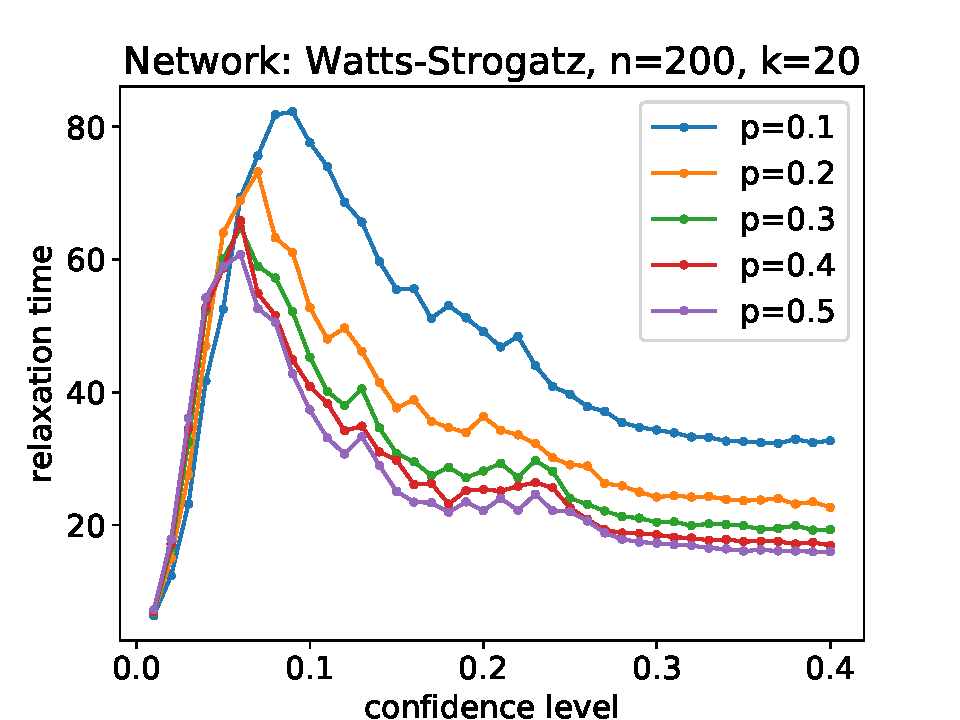
\includegraphics[width=0.7\textwidth]{/home/arti/studia/python/praca_magisterska/plots/steps_Watts-Strogatz_n=200_k=20.pdf}
		\caption{Average relaxation time for Watts--Strogatz network with $n=200$, $k=20$ as a function of confidence level for various values of $p$.}
		\label{f33}
\end{figure}

For confidence level big enough (in this case at least $\epsilon=0.08$) networks with small value of parameter $p$ relax much slower. For example when $\epsilon=0.20$ network with $p=0.5$ relax in time $t=22$, while network with $p=0.1$ relax in $t=49$ (more than twice slower). When Watts--Strogatz network has regular topology (agents change their initial neighbors rarely), changes in opinions walk slowly through network, because path between two agents from different network regions is long.

\indent

In Fig. \ref{f34}, results for BA networks are shown.

\begin{figure}[H]
		\centering
		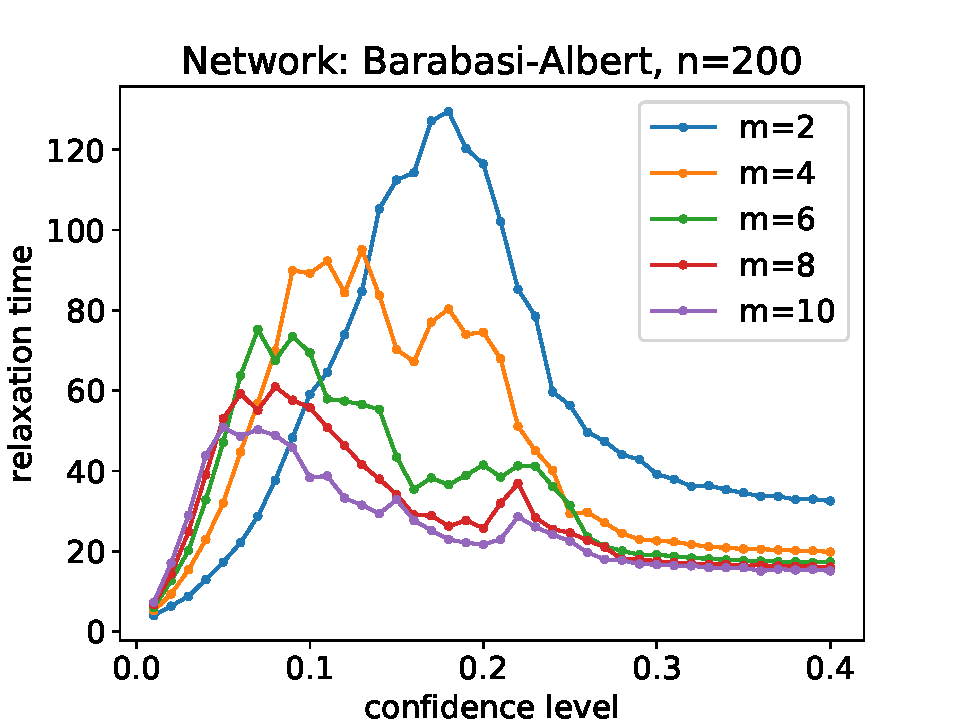
\includegraphics[width=0.7\textwidth]{/home/arti/studia/python/praca_magisterska/plots/steps_Barabasi-Albert_n=200.pdf}
		\caption{Average relaxation time for Barabasi--Albert network with $n=200$ as a function of confidence level for various values of $m$.}
		\label{f34}
\end{figure}

The bigger is the value of parameter $m$, the faster a network achieve the peak value of the average relaxation time. Firstly, the relaxation times increase with $\epsilon$, because bigger the confidence level, the more new influential connections appear in the course of time. Then, they decrease because when $\epsilon$ is big enough agents   change their opinions more in first few MCS and networks relax quicker. We observe additionally second small peaks of relaxation times, when:
\begin{itemize}
\item $\epsilon=0.18$ for $m=4$,
\item $\epsilon=0.22$ for $m=6,8,10$.
\end{itemize}

They emerge due to phase transition from polarization to consensus. 
For small confidence level, e.g. $\epsilon=0.05$ weak--connected networks ($m=2,4$) relax much faster than networks with more connections ($m=6,8,10$). It happens so, because not much changes in agent opinions when $m$ and $\epsilon$ are small (see Figure \ref{acba}). Above $\epsilon=0.15$ the behavior is different -- the bigger $m$, the faster relaxation. Due to bigger number of connections, more agents can influence each other in one MCS, hence the system relax faster. 

\indent

We conclude this section with a direct comparison of different networks (Fig. \ref{f35}).

\begin{figure}[H]
		\centering
		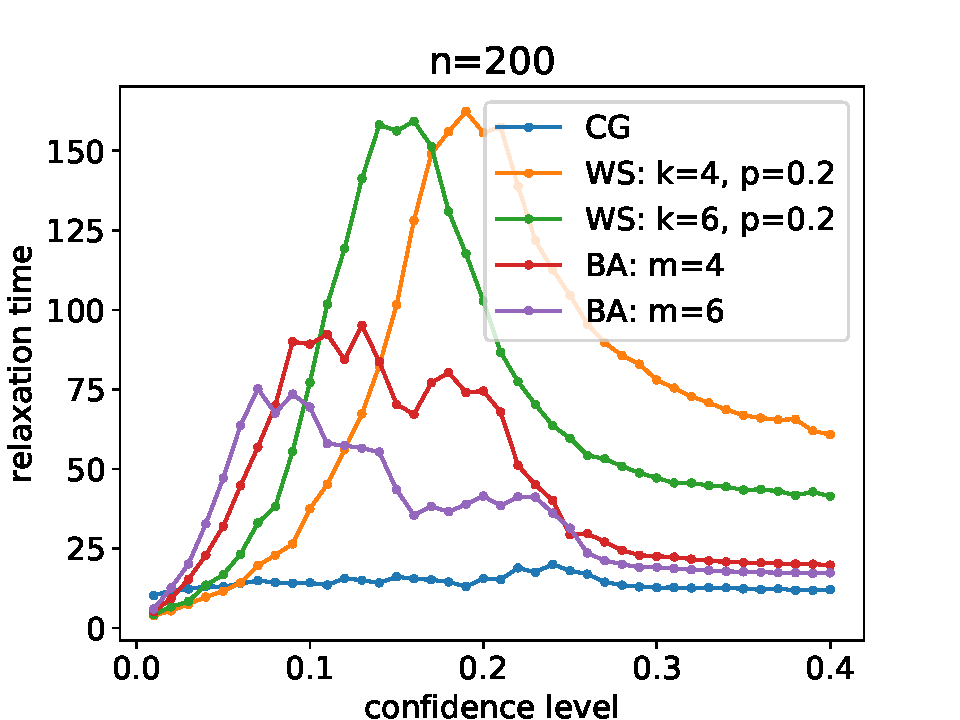
\includegraphics[width=0.7\textwidth]{/home/arti/studia/python/praca_magisterska/plots/steps_various.pdf}
		\caption{Average relaxation time for various networks with $n=200$ as a function of confidence level.}
		\label{f35}
\end{figure}

Except very small values of $\epsilon$, the WS networks relax much longer than the others. It is the consequence of non--centralized topology of them, especially when $p$ is small, like in the case $p=0.2$. In those networks the path between two agents from different regions is long and as a consequence it takes more time for opinions to spread.

\section{Summary}

From the conducted simulations and obtained results we see that all investigated parameters such as:
\begin{itemize}
\item $\epsilon$ -- confidence level,
\item $n$ -- network size,
\item $k$ -- number of agent neighbors in Watts--Strogatz network,
\item $p$ -- probability of changing neighbor in Watts--Strogatz network,
\item $m$ -- number of new agent connections in Barabasi--Albert network,
\end{itemize}
can influence the opinions dynamics process of BC model. 

\indent

As we described in section about network topologies, various types of networks may be used to various cases of opinions formation problems. As it turns out, topology of considered network has great impact on how agents interact and change their opinions. To sum up the results, we will briefly go through the most important ones.

\indent

For a given confidence level Watts--Strogatz and Barabasi--Albert networks are more eager to reach consensus than complete graph network. Moreover the most consensus--likely networks are weak--connected ones, as small number of connections favors gradual opinion changing which lead to agreement.

Of course consensus is not the only possible result of opinion dynamics. Final opinions of agents typically change from fragmentation, through polarization to consensus as confidence level increases. Polarization of opinions is the most likely to occur in complete graph network and also in Barabasi--Albert on the condition that it is well--connected (typically for $0.15 \leq \epsilon \leq 0.20$). Watts--Strogatz network with small number of agents' connections and regular layout is less likely to polarize and rather dynamically changes from fragmentation to consensus as confidence level increases. In weak--connected Barabasi--Albert network polarization emerge more likely because of the centralized network structure.

Network structure is also important, when we concern number of main clusters sharing one common opinion. Small confidence levels (up to $\epsilon=0.1$) lead to bigger fragmentation for weak--connected Barabasi--Albert and Watts--Strogatz networks than for well--connected networks, whereas large confidence levels ($\epsilon>0.15$) lead to opposite behavior.

As the matter of fact, not only the network structure, but also the size of the network have impact on final state of the system. For all network topologies the bigger is the network size, the faster (in terms of confidence level) agents reach consensus, also phase transition from polarization to consensus is more concentrated around one point for bigger networks, in the complete graph case this point is $\epsilon\approx0.22$.

Even when the majority of agents in a network share one common opinion, still some of individuals might not change their opinions at all. In weak--connected Barabasi--Albert and Watts--Strogatz networks extreme opinions are much more likely to survive than in complete graph networks when confidence level is big. This happens when an agent who has an extreme opinion does not have any neighbors inside his confidence interval and hence he does not change his initial opinion at all.

However, in most of the cases agents interact with others. They change opinions the most usually at the beginning of opinions dynamics process, the process is the most stretched in time for Watts--Strogatz networks with regular layout (small $p$) due to big values of average path lengths. Complete graph networks have the shortest relaxation times.

Sometimes relaxation time increases when confidence level is such that network hesitates between polarization and consensus, especially when network is well--connected.

\newpage

\begin{thebibliography}{90}

\bibitem{sp}
C. Castellano, S. Fortunato, V. Loreto 
	\emph{Statistical physics of social dynamics}. Rev. Mod. Phys. 81, 591 (2009)

\bibitem{qv} 
C. Castellano, M.A. Munoz, R. Pastor-Satorras
  \emph{The non-linear q-voter model}.  
Physical Review E 80, 041129 (2009)

\bibitem{mr} 
S. Galam
	\emph{Minority opinion spreading in random geometry}.
Eur. Phys. J. B 25, 403-406 (2002)

\bibitem{sm}
K. Sznajd-Weron, J. Sznajd
	\emph{Opinion evolution in closed community}. Int. J. Mod. Phys. C 11, 1157 (2000)
	
\bibitem{dm}
G. Deffuant, D. Neau, F. Amblard, G. Weisbuch
	\emph{Mixing beliefs among interacting agents}. Adv. Compl. Sys. 3(1-4), 87 (2000)
	
\bibitem{bc}
R. Hegselmann, U. Krause
	\emph{Opinion dynamics and bounded confidence: models, analysis and simulation}. JASSS 5(3) (2002)

\bibitem{cg}
J.M. Harris, J.L. Hirst, M.J. Mossinghoff
	\emph{Combinatorics and Graph Theory}.
Undergraduate Texts in Mathematics, Springler (2008)

\bibitem{ws}
D. Watts, S. Strogatz
	\emph{Collective dynamics of ‘small-world’ networks}.
Nature vol. 393, 440–442 (1998)

\bibitem{ba}
A. L. Barabási, R. Albert
	\emph{Emergence of scaling in random networks}.
Journal Science vol. 286, 5439, 509-512 (1999)

\bibitem{kiss}
T. Terano
	\emph{Beyond the KISS principle for agent-based social simulation}. Journal of
Socio-informatics 1, 175–187 (2008)

\bibitem{sai}
P. Sen, B. K. Chakrabarti
	\emph{Sociophysics: An Introduction}.
OUP Oxford, 283 (2014)


\end{thebibliography}

\end{document}